\documentclass[a4paper]{article}

%% Language and font encodings
\usepackage[english]{babel}
\usepackage[utf8x]{inputenc}
\usepackage[T1]{fontenc}

%% Sets page size and margins
\usepackage[a4paper,top=3cm,bottom=2cm,left=3cm,right=3cm,marginparwidth=1.75cm]{geometry}

%% Useful packages
\usepackage{amsfonts, amsmath, amssymb, nicefrac}
\usepackage{graphicx}
\usepackage{wrapfig}
\usepackage[colorinlistoftodos]{todonotes}
\usepackage[colorlinks=true, allcolors=black]{hyperref}

\setlength{\parskip}{1.5ex plus0.5ex minus0.5ex}
\setlength{\parindent}{0em}
\setlength{\headheight}{15pt}
\setlength{\headsep}{30pt}
\setlength{\marginparwidth}{2cm}
\renewcommand{\floatpagefraction}{.8}
 
\title{Best Laid Plans of Lions and Men}
\author{Danny-Marvin Rademacher, Jens Harder}
\date{11.10.2017}

\begin{document}
\maketitle

%%%%%%%%%%%%%%%%%%%%%%%%%%%%%%%%%%%%%%%%%%%%%%%%%%%%%%%%%%%%%%%
%%                                                           %%
%%                                                           %%
%%  https://www.overleaf.com/10975949ttqhccgxsxmn#/41322390/ %%
%%                                                           %%
%%                                                           %%
%%%%%%%%%%%%%%%%%%%%%%%%%%%%%%%%%%%%%%%%%%%%%%%%%%%%%%%%%%%%%%%

% \newpage
% \tableofcontents
% \newpage

\begin{abstract}
During the lab `Computational Geometry` (SS 2017) in the University of Bonn we designed an applet to visualize
the algorithm in the paper `Best Laid Plans of Lions and Men`. This paper describes two different configurations for the Men and Lions Problem. The first configuration has a bounded area which is transformed into a discrete graph. The second configuration uses men and lions in the reel plane. The work is a visualization of both problems and the described algorithms so that people can use them in teaching and for research purposes. Furthermore we extended the problem settings on the graph with additional algorithms and configuration parameters to explore more characteristics of the problem.
\end{abstract}

%  \section{Introduction}


This documentation gives a short overview over the problems and an explanation of the applet and its functionalities.

\section{Lions and Men Problem}

In the Lions and Men Problem, $n$ lions try to catch $m$ men in a special environment. The men try to escape as long as possible, against all possible lion strategies. \cite{paper} gives for two different environments (special graph and plane) man strategies to escape always all lions.

\subsection{On a graph}

The first configuration describes a special designed graph and an algorithm such that one man can always escape two lions, independent of the lion strategies.

In this special graph (see figure \ref{fig:specialGraph}) each vertex has 3 incident edges and each edge has weight 4. This means that an entity (man or lion) needs 4 steps to run from one vertex to one of the neighbor vertices. A \textit{quarter} of an edge is an edge step which is next to a vertex. 

The man runs from \textit{quarter} to \textit{quarter} and decides with only the current lion positions, where to go next (without knowing the future steps of the lions).


\begin{figure}[!hbt]
  \centering
    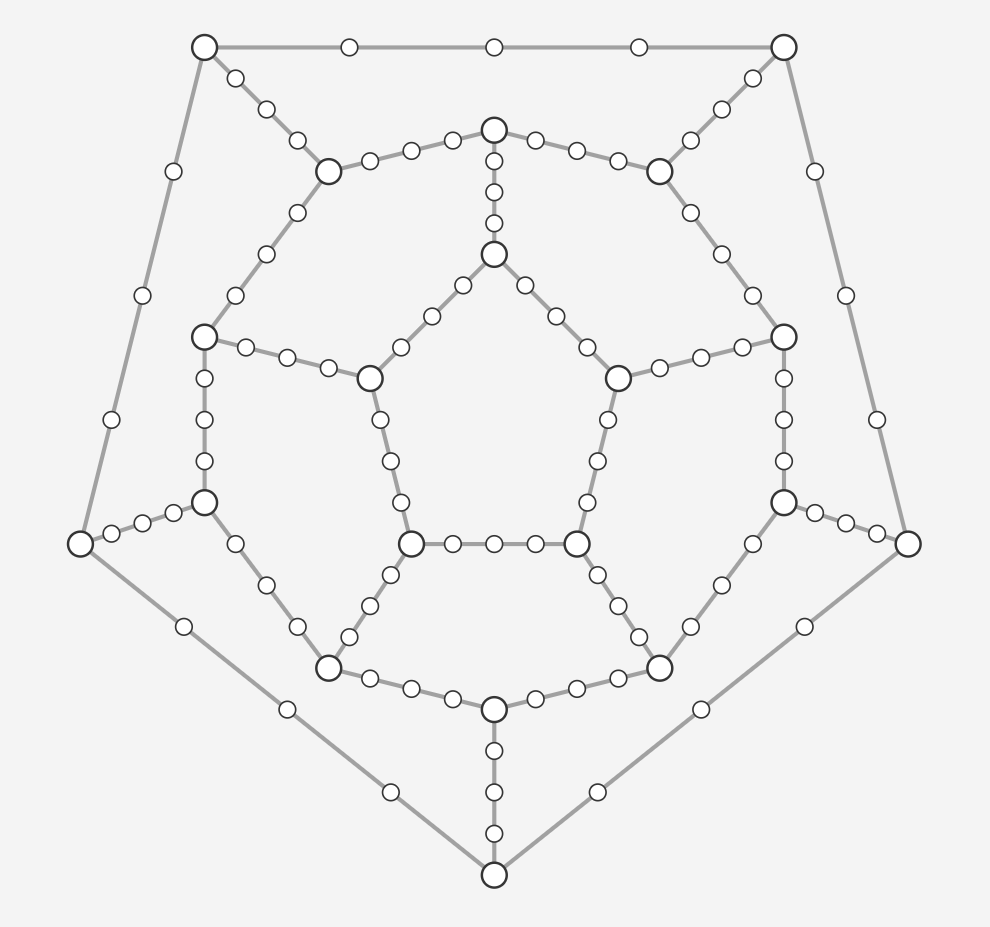
\includegraphics[width=0.55\textwidth]{specialGraph.PNG}
  \caption{Special designed graph in \cite{paper}}
  \label{fig:specialGraph}
\end{figure}

\subsection{In the plane}

This configuration is in the $\mathbb{R}^2$ plane. All n lions move around the plane with speed $1$ to catch one man. The man has speed $1 + \epsilon$ with $\epsilon > 0$.

\cite{paper} provides an algorithms, in which the man can always escape the lions, if the starting position of all lions is different to the starting position of the man. The goal is to escape from all lions. Since the man has a higher speed than all lions it is sufficient to be outside the convex hull.
The idea of the algorithm is to induce over all lions and build up the escape path from the previous path and the behavior of the lion. The induction base of the algorithm is trivial. The man runs in the opposite direction of the lion and escapes. 

The induction step of the algorithm works as following. It starts with the path given by the induction hypothesis. That path is an escaping path on the old lion set. If the new lion is not able to interfere with the escaping path, the new man path is the same as the old path. If the new lion is interfering the escaping path the man has to make alterations to the given path in order to maintain a path escaping the lions. This is done by having a procedure with is called the avoidance move. That move is a counterclockwise arc around the lion. Once the move has passed the lion, the man continues on the original path. Then we know that that path is an escaping path by induction hypothesis. It is important, that the man gets more speed each induction step (to at most $1 + \epsilon$ speed).


\section{The Applet}
When starting the applet, you get to the main screen where you can choose which part of the applet to use. There are to different parts: the "Lions On Graph" part (section \ref{sec:applet_graph}) and the problem "Lions In Plane" (section \ref{sec:applet_plane}). You can switch between both parts any time, using the "Choose App" button in the bottom right corner.

\begin{figure}[hbt]
  \centering
    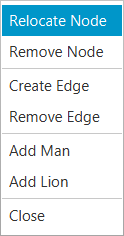
\includegraphics[width=0.25\textwidth]{modify.png}
  \caption{Modify a graph}
  \label{fig:modify}
\end{figure}

\subsection{Lions On Graph}\label{sec:applet_graph}

\subsubsection*{Create and modify the graph}

% \begin{wrapfigure}{r}{0.36\textwidth}
%   \vspace{-20pt}
%   \begin{center}
%     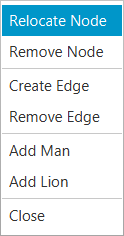
\includegraphics[width=0.25\textwidth]{modify.png}
%   \end{center}
%   \vspace{-20pt}
%   \caption{Modify a graph}
%   \label{fig:modify}
%   \vspace{-10pt}
% \end{wrapfigure}

If you choose "Lions In Plane", you see an empty screen. With "Set Graph" you can open an existing graph, load a graph file (if available), or create your own graph. It is possible to create or modify the graph manually with right clicks. To create a new vertex, click on an emtpy place and choose "Add Node". To relocate or remove vertices, do a right click on the vertex (figure \ref{fig:modify}). Edges can be created or removed with right clicks as well. Click on the starting vertex, choose "Create Edge" and click on the end vertex of the edge you want to create.

\subsubsection*{Create and modify the entities}
To create, remove or relocate entities (lions and men), do a right click on a vertex or on the entity itself. Furthermore you can change the entity properties such as the strategy or the range. Just click on the property and select or insert the new value.

\begin{figure}[hbt]
  \centering
    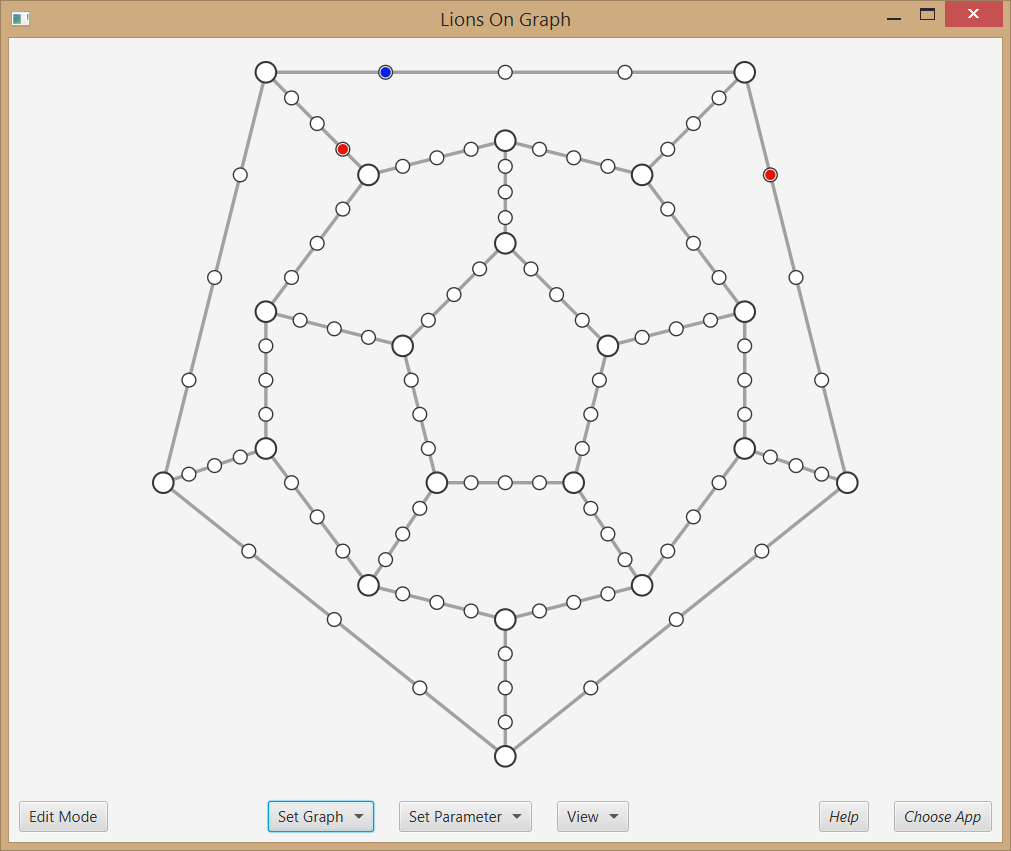
\includegraphics[width=0.75\textwidth]{graphApplet.PNG}
  \caption{Example Configuration. The special graph from \cite{paper} with one man (blue) and two lions (red).}
  \label{fig:graphApplet}
\end{figure}

\subsubsection*{Usage}
After you created the graph with the entities (figure \ref{fig:graphApplet}), you can go to the "Play Mode" (bottom left corner).
\begin{figure}[hbt]
  \centering
    
\includegraphics[width=0.75\textwidth]{play.PNG}
  \caption{Different play options}
  \label{fig:play}
\end{figure}
In the "Play Modus", you can start the complete animation ("Play"), do the animation step by step ("Single Step") or change the animation speed. You can also change which parts of the entities should be visible. See figure \ref{fig:play}.\\
If one of the strategies is "Manual" you can choose each step where to move this entity. Note: During the "Play Mode" it is not possible to change entity properties (such as the strategy) or to modify the graph. To change the setup you need to go back to the "Edit Mode" (bottom left corner)

\subsection{Lions In Plane}\label{sec:applet_plane}

\subsubsection*{Create and modify the plane}
Analogous to the "Lions On Graph" applet, you can modify the plane with right clicks. Right click on a empty place you can add a new lion or the man. With a right click on an entity you can relocate the entity or change the strategy. If you added multiple lions, you can see the green polygon which is the convex hull of all lions. To escape all lions, the man needs to escape from the convex hull. This is enough, because the man is $\epsilon > 0$ faster then the lions.

\subsubsection*{Usage}
If you created all lions and the man (see figure \ref{fig:planeApplet}), you can go to the "Play Mode" (bottom left corner).

In the "Play Modus", you can start the complete animation ("Play"), do the animation step by step ("Single Step") or change the animation speed. You can also change which parts of the entities should be visible.\\

\begin{figure}[hbt]
  \centering
    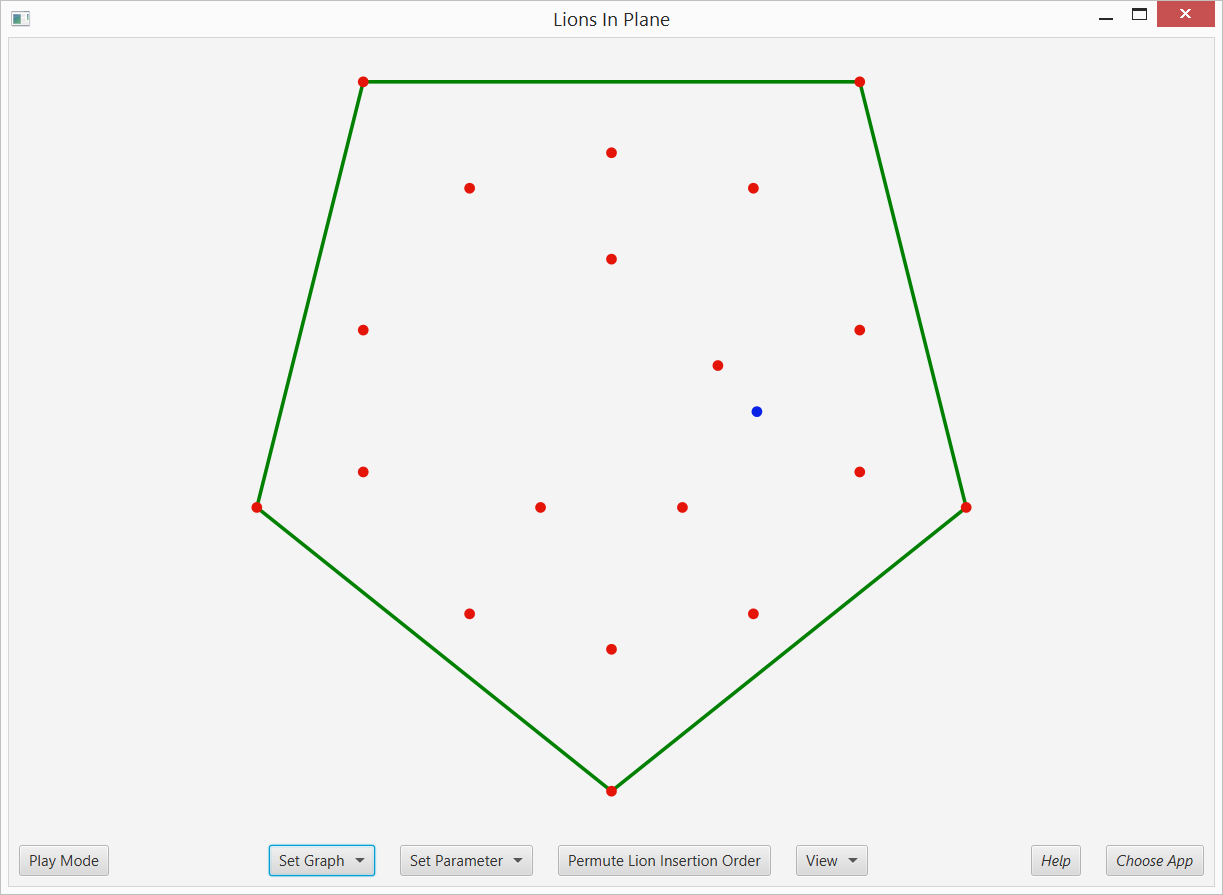
\includegraphics[width=0.75\textwidth]{planeApplet.PNG}
  \caption{Example Configuration. The plane with one man (blue) and multiple lions (red). You can see the convex hull of the lions (green)}
  \label{fig:planeApplet}
\end{figure}
\begin{figure}[hbt]
  \centering
    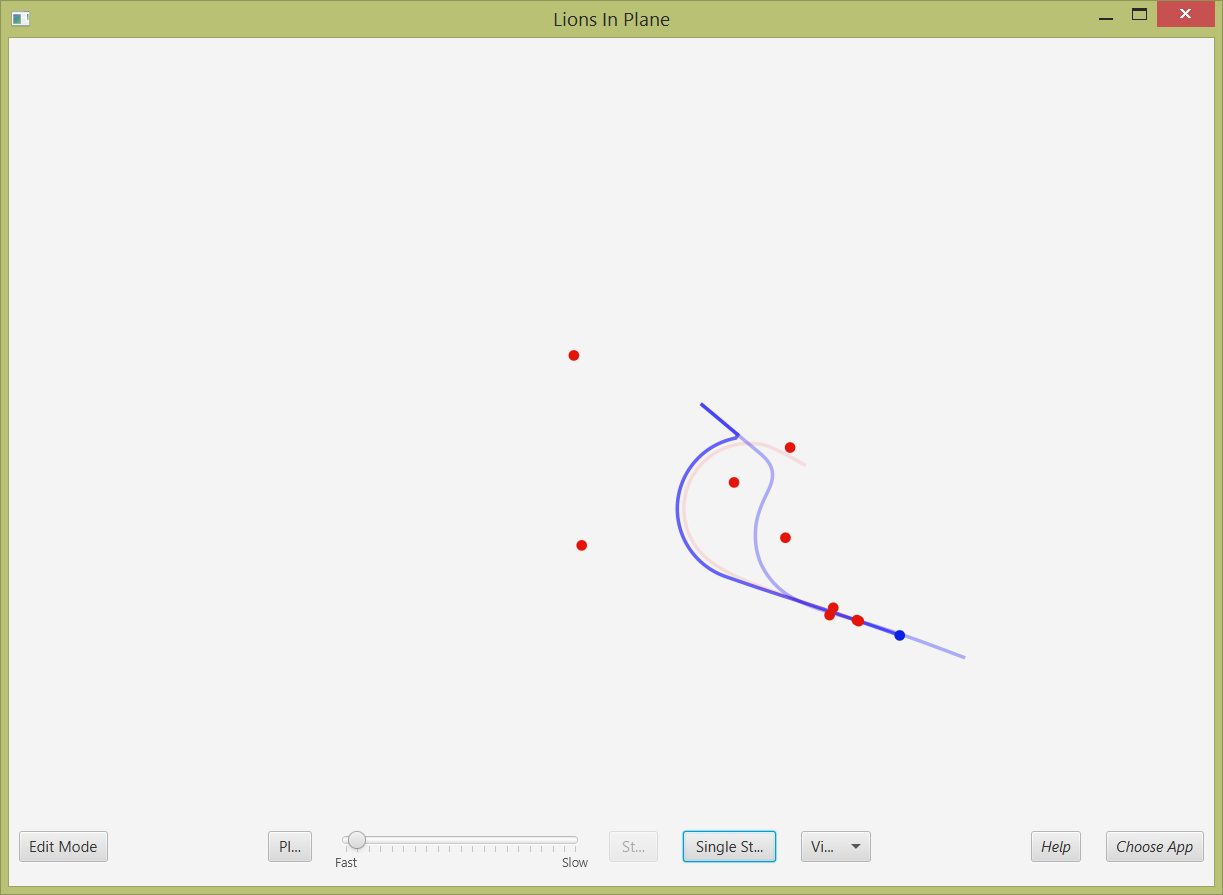
\includegraphics[width=0.75\textwidth]{planeAppletRun.PNG}
  \caption{During the animation. You can see the man path from the last induction step (light blue), the man path from the current induction step (blue) and the lion path from the current lion (light red). All lions are red points and the man is the blue point.}
  \label{fig:planeAppletRun}
\end{figure}

With "View" you can decide which shapes / paths should be visible in the applet. During the animation, the applet shows each induction step, until the induction over all lions is completed (see figure \ref{fig:planeAppletRun}). Note: Is is not possible to add, remove or change entities in the "Play Mode". You have to go back to the "Edit Mode" to modify the setup.



\newpage
%	\defaultsectionstyle	
	\begin{thebibliography}{99}
		
		
		\bibitem[Ab17]{paper} \textsc{M. Abrahamsen, J. Holm, E. Rotenberg, C. Wulff-Nilsen} (2017): Best Laid Plans of Lions and Men. (SOCG'17) arXiv:1703.03687 [cs.CG]

	

		
	\end{thebibliography} 



\end{document}